\documentclass{article}
\usepackage{amsmath}
\usepackage{graphicx}
\usepackage{tikz}
\usepackage{amsmath}

\title{Datenaufteilung}
\author{}
\date{}

\begin{document}

\maketitle

\section*{1}

\subsection*{1.1 Generische Formel}

\[
\text{Matrixgröße} = (8 \cdot i + 9) \times (8 \cdot i + 9)
\]

\[
\text{Zeilen pro Thread} = \left\lfloor \frac{8 \cdot i + 9}{t} \right\rfloor
\]

\subsection*{1.2 Konkrete Aufteilungen}

\begin{tabular}{|c|c|c|c|}
\hline
$i$ & $t$ & Thread-ID & Daten-Grenzen \\
\hline
0 & 1 & 0 & 0 - 8 \\
\hline
0 & 3 & 0 & 0 - 2 \\
  &   & 1 & 3 - 5 \\
  &   & 2 & 6 - 8 \\
\hline
0 & 12 & 0 & 0 - 0 \\
  &    & 1 & 1 - 1 \\
  &    & 2 & 2 - 2 \\
  &    & 3 & 3 - 3 \\
  &    & 4 & 4 - 4 \\
  &    & 5 & 5 - 5 \\
  &    & 6 & 6 - 6 \\
  &    & 7 & 7 - 7 \\
  &    & 8 & 8 - 8 \\
\hline
1 & 3 & 0 & 0 - 5 \\
  &   & 1 & 6 - 11 \\
  &   & 2 & 12 - 16 \\
\hline
\end{tabular}

\section*{1.3 Visualisierung}

\subsection*{Matrix für $(i=0, t=3)$}

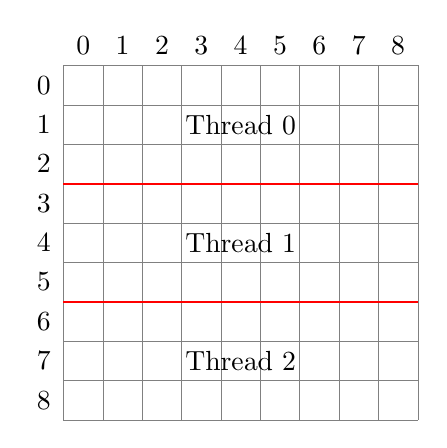
\begin{tikzpicture}
    % Zeichne das Gitter
    \draw[step=0.5cm,gray,very thin] (0,0) grid (4.5,4.5);

    % Beschriftung für die X-Achse (oben)
    \foreach \x in {0,1,...,8} {
        \node at (\x*0.5+0.25,4.75) {\x}; % Nach oben verschoben (Y-Koordinate leicht erhöht)
    }

    % Beschriftung für die Y-Achse (links)
    \foreach \y in {0,1,...,8} {
        \node at (-0.25,4-\y*0.5+0.25) {\y}; % Position bleibt gleich
    }

    % Rote Linien
    \draw[thick,red] (0,3) -- (4.5,3);
    \draw[thick,red] (0,1.5) -- (4.5,1.5);

    % Beschriftung für Threads
    \node at (2.25,3.75) {Thread 0};
    \node at (2.25,2.25) {Thread 1};
    \node at (2.25,0.75) {Thread 2};
\end{tikzpicture}

\subsection*{Matrix für $(i=1, t=3)$}

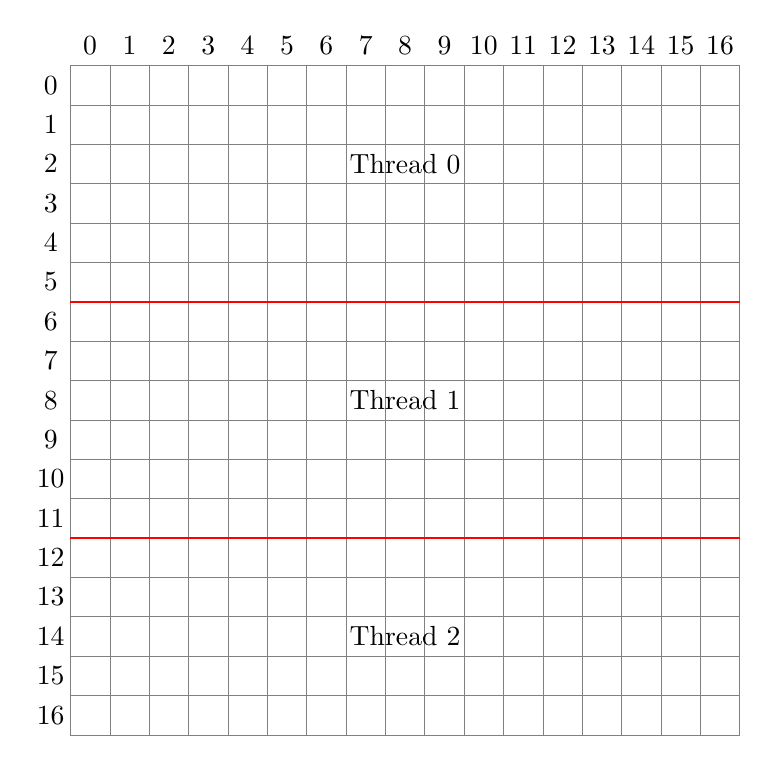
\begin{tikzpicture}
    \draw[step=0.5cm,gray,very thin] (0,0) grid (8.5,8.5);
    \foreach \x in {0,1,...,16} {
        \node at (\x*0.5+0.25,8.75) {\x};
        \node at (-0.25,8-\x*0.5+0.25) {\x};
    }
    \draw[thick,red] (0,5.5) -- (8.5,5.5);
    \draw[thick,red] (0,2.5) -- (8.5,2.5);
    \node at (4.25,7.25) {Thread 0};
    \node at (4.25,4.25) {Thread 1};
    \node at (4.25,1.25) {Thread 2};
\end{tikzpicture}

\newpage
\subsection*{1.4 Pseudocode}

\begin{verbatim}
function distributeMatrix(matrix, i, t):
    N = 8 * i + 9
    rows_per_thread = floor(N / t)
    for thread_id in range(t):
        start_row = thread_id * rows_per_thread
        end_row = (thread_id + 1) * rows_per_thread - 1
        if thread_id == t - 1:
            end_row = N - 1
        assignRowsToThread(thread_id, start_row, end_row)

function calculateStar(matrix, options):
    for thread_id in range(t):
        start_row, end_row = getThreadRows(thread_id)
        for i in range(start_row, end_row + 1):
            for j in range(1, N - 1):
                star = 0.25 * (matrix[i-1][j] + matrix[i]
                [j-1] + matrix[i][j+1] + matrix[i+1][j])
                if options.inf_func == FUNC_FPISIN:
                    star += fpisin_i * sin(pih * j)
                matrix[i][j] = star
\end{verbatim}

\end{document}